Risk analysis is a process which enables the analysis of risks, associated
within  a project. A Risk can be generally defined as the probability of
something going wrong, and the negative consequences if it does. However, it is
hard to find all the risks, which can occur, in a project. At first it should be
recognised that a risks exists as a consequence of uncertainty. For this reason
the risk analysis process will help to identify potential problems that may
occur. Such a risk analysis can be useful in several situations: 
\begin{itemize}
\item To help to anticipate and neutralise possible problems when planning
projects.
\item To decide wether to continue with the project or not.
\item To improve safety and manage potential risks in the workplace.
\end{itemize}


\section{Identifying the Risks}
As one of the first steps in Risk Analysis it is to identify the existing and
possible problems occur. Some of these areas and threats, which might have an
impact on this project, are listet below:
\begin{itemize}
\item Project Members -- Illness, injury, or another reason leading to a loss of
a project member.
\item Operational �- Delays in deliveries.
\item Reputational �- Loss of customer or employee confidence.
\item Project �- Taking too long on concluding key tasks, or experiencing
issues with product or service quality, goal not achieved.
\item Financial �- Budget exhausted, Business failure or non-availability of
funding.
\end{itemize}

\section{Estimate Risks}
After some of the possible threats has been faced, the risk can be calculated
with both the likelihood of these threats being realised, and their possible
impact. One way of doing this is to make a estimation of the probability that
this threat occurrs multiplied by the amount it will cost. This leads to the
following equation which quantifies the risk:
\begin{equation}
Risk = Probability\,of\, Occurance \cdot Cost
\end{equation}
Additionally there are two possible kinds of processes:
\begin{itemize}
\item The total value of a risk of a series of processes that are executed
successively can be calculated as follows:
\begin{equation}
R_{Total} = R_{n} \cdot R_{n+1}
\end{equation}
\item The total value of a risk of parallel processes that are executed
concurrent can be calculated as follows:
\begin{equation}
R_{Total} = 1 - (1-R_{n}) \cdot (1 - R_{n+1})
\end{equation}
\end{itemize}

As an example the risk value of an illness of a project member will be
calculated. The estimated propbillity will be set to 0.4. Lets assume that the
member is ill for about a week. One day has 8 working hours and the salary
for this member would be 50\pounds \,per hour. 
\begin{equation}
Risk = Probability\,of\, Occurance \cdot Cost = 0.4 \cdot 5 \cdot 8 \cdot
50\pounds = 800\pounds
\end{equation}
So the risk value for this threat would be 800\pounds. 

In order to determine what risks to focus on, an Impact / Probability Chart can
be very useful. An Impact / Probability Chart is a two dimensional diagram
whereat on the axis of ordinates the probability of Occurrence will be plotted
and on the axis of abscissas the impact on the project. For this purpose, a
probability and the associated impact are assigned to the identified risks.
However, this is carried out only by way of example at a respective risk from
each area and then drawn into the diagram. The assigned probabilities and
impacts can taken from the following table.

\begin{table}[h!]
  \centering
    \footnotesize
\begin{adjustbox}{max width=\textwidth}
\begin{tabular}{c|c|c}
Risk&Probability&Impact\\
\hline
\hline
Illness of Project Member&0.4&3\\
Delay in Deliveries&0.35&8\\
Loss of Customer Confidence&0.5&7\\
Specified Goals not achieved&0.7&9\\
Budget exhausted&0.2&10\\
\end{tabular}
\end{adjustbox}
\captionsetup{justification=centering}
  \caption{Frequency analysis Novel}
  \label{tab:frequency analysis novel}
\end{table}

The following figure shows an exemplarily Impact / Probability Chart with the
estimated probabilities and associated impacts on the project:

\begin{figure}[h!]
  \centering
     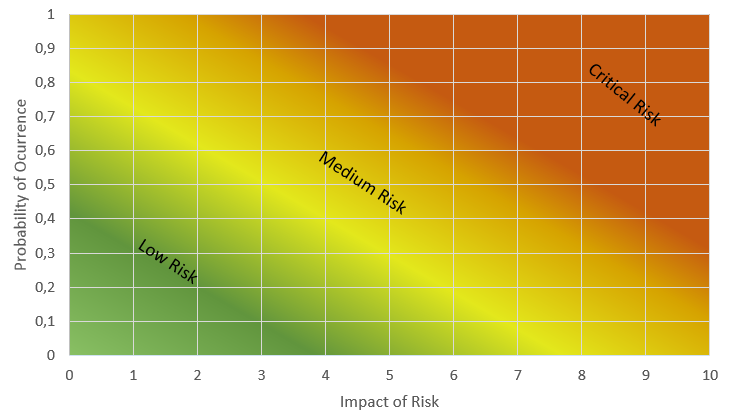
\includegraphics[width=1\textwidth,
     height=0.4\textheight]
     {res/impactchart.png}
     \captionsetup{justification=centering}
  \caption{Impact / Probability Chart}
  \label{fig:ImpactChart}
\end{figure}

\FloatBarrier

As it can be seen, the chart has several areas. With help of this areas it can
be figured out, if the the risk has priority or not. The characteristics of
these areas will be explained subsequently:

\begin{itemize}
\item Low impact/low probability - risks in this area can often be ignored.
\item Low impact/high probability � these risks are of moderate importance but
they have to be noticed and it should be tried to avoid that they occure
\item High impact/low probability - these are of high importance and should not
occure because the probablility is very low. If so, a contingency plans should
be available.
\item High impact/high probability � risks in this area are of critical
importance and have the highest priority.
\end{itemize}

On the basis of this Impact / Probability Chart, the main focus should be on the achievement
of the goals, as these have the highest priority.


\section{Dealing with Risks}

To successfully execute a project, the risks has to be identified. Afterwards
the focus has to be on the middle and high-priority risks. Otherwise resources
on unecessary risks will be a waste. Since the risks has been identified and
prioritised, the next step is how to deal with them. The following is a brief
discussion of four different ways of dealing with risks.

\subsection{Risk Avoidance}
The aim of risk avoidance is to avoid any risk, even if they are very small. The
suggestion of maximum safety through very strong differentiation and a high
control is at the expense of free processes. An example related to the project
is the early planning of the tasks and the associated aims. Through very strict
planning it is already tried in the run-up to avoid all risks, to transfer them
or to turn activities so that risks can not occur. All these actions are at the
expense of project budgets and scheduling but in favor of quality.

The idea of risk avoidance: ``do not take any risks'' means maximum security
while at the same time avoiding opportunities, including rejecting cooperation with
certain partners and a longer project run-time with higher costs.

\subsection{Risk Reduction}
Risk reduction means that through various procedures in the field of personnel
organisation and workplace organisation attempts are made to keep the specific
probability of occurrence of the risks as small as possible. Examples for this
could be, point explicitly to the risks of the respective task to the project
members and communicate the risks transparent to all project members so that a
shared understanding can be achieved.

The idea of risk reduction: by means of personnel processes (training,
qualification, involvement of experts) and technical processes (only processing
quality materials, making processes and optimising them), permanently reduce the
probability of occurrence of risks.

\subsection{Risk Transfer}

During the transfer, risks are passed on to third parties through contracts and
/ or the assignment of service providers. If, for example, many risks occur
during a project phase, it can be considered to outsource the entire task to a
partner.

The idea of risk transfer: through service-level agreements, contracts or
outsourcing, the risks and any related tasks are completely and in writing
passed to third parties, which can then be made liable for a risk entry.

\subsection{Risk Acceptance}
The idea of risk acceptance: risks with very low scope and very low probability
of occurrence, as well as risks that can not be circumvented, should be accepted as such.

\section{Conclusion}
In this chapter it has been worked out what risks are and how they can be
identified. It was then shown how the risk value can be calculated from the
costs and the probability of the occurrence. Afterwards, the identified risks
were prioritized using the Impact / Probability Chart and the handling of risks
was dealt with most recently.

Finally, the further the project progresses, the lower the risk.